% Tamaño de letra.
\documentclass[12pt,titlepage]{article}

%------------------------------ Paquetes ----------------------------------

% Paquetes:

%Para comentarios multilínea.
\usepackage{verbatim}

% Para tener cabecera y pie de página con un estilo personalizado.
\usepackage{fancyhdr}

% Codificación UTF-8
\usepackage[utf8]{inputenc}

% Castellano.
\usepackage[spanish]{babel}

% Tamaño de página y márgenes.
\usepackage[a4paper,headheight=16pt,scale={0.75,0.8},hoffset=0.5cm]{geometry}

% Para poder agregar notas al pie en tablas:
%\usepackage{threeparttable}

% Tipo de letra Helvetica (Arial).
%\usepackage{helvet}
%\renewcommand\familydefault{\sfdefault}

% Gráficos:

% Para incluir imágenes, el siguiente código carga el paquete graphicx
% según se esté generando un archivo dvi o un pdf (con pdflatex).

% Para generar dv.
%\usepackage[dvips]{graphicx}

% Para generar pdf.
\usepackage[pdftex]{graphicx}
\pdfcompresslevel=9

%
% Directorio donde están las imagenes.
%
%\newcommand{\imgdir}{includes}
%\graphicspath{{\imgdir/}}

%------------------------------ ~paquetes ---------------------------------

%------------------------- Inicio del documento ---------------------------

\begin{document}

% ---------------------- Encabezado y pie de página -----------------------

% Encabezado: sección a la derecha.
% Pie de página: número de página a la derecha.

\pagestyle{fancy}
\renewcommand{\sectionmark}[1]{\markboth{}{\thesection\ \ #1}}
\lhead{}
\chead{}
\rhead{\rightmark}
\lfoot{}
\cfoot{}
\rfoot{\thepage}

% ---------------------- ~Encabezado y pie de página ----------------------

% -------------------------- Título y autor(es) ---------------------------

\title{Concu-chat}
\author{}

% -------------------------- ~Título y autor(es) --------------------------

% ------------------------------- Carátula --------------------------------

\begin{titlepage}

\thispagestyle{empty}

% Logo facultad más pie de la figura.
\begin{center}

\includegraphics[scale=0.55]{./Images/fiuba}\\
\large{\textsc{Universidad de Buenos Aires}}\\
\large{\textsc{Facultad De Ingeniería}}\\
\small{Año 2010 - 1\textsuperscript{er} Cuatrimestre}
\end{center}

\vfill

% Título central.
\begin{center}

\Large{\underline{\textsc{Técnicas de programación concurrente (75.59)}}}

\vfill

% Tabla de integrantes.

\Large{\underline{\textsc{Trabajo Práctico: Concu-Chat}}}

\vfill
 
\Large\underline{Integrantes} \linebreak\linebreak

% Separación entre columnas.
\large\addtolength{\tabcolsep}{-3pt}
% Tres columnas con alineación centrada.
\begin{tabular}{|| c | c | c ||}
\hline
\textbf{Apellido, Nombre} & \textbf{Nro. Padrón} & \textbf{E-mail} \\
\hline
Ferreiro, Demian & 88443 & epidemian@gmail.com \\
\hline
Mouso, Nicolás Gastón & 88528 & nicolasgnr@gmail.com \\
\hline
\end{tabular}
\end{center}

\vfill

\hrule
\vspace{0.2cm}

% Pie de página de la carátula.
\noindent\small{75.59 - Técnicas de programación concurrente\hfill Grupo 4}

\end{titlepage}

% ------------------------------- ~Carátula -------------------------------

% -------------------------------- Índice ---------------------------------

% Hago que las páginas se comiencen a contar a partir de aquí.
\setcounter{page}{1}

% Índice.
\tableofcontents
\newpage

% -------------------------------- ~Índice --------------------------------

% ----------------------------- Inicio del tp -----------------------------

\section{Enunciado}

\subsection*{Objetivo}

El objetivo de este trabajo es el desarrollo de un sistema de chat conocido como ''ConcuChat".  Este 
es un sistema que permitirá a dos partes poder chatear mediante el intercambio de mensajes 
instantáneos.  Esto quiere decir que ambas partes podrán comunicarse únicamente si ambas están 
''en línea".

\subsection*{Arquitectura}

El sistema deberá estar formado por los siguientes módulos:

\begin{enumerate}
  \item Servicio de Localización
  \item Programa de Chat
\end{enumerate}

\subsection*{Servicio de Localización}

Es un módulo que se encarga de almacenar el nombre y la dirección de los distintos programas de 
chat que estén en ejecución, así como de realizar la resolución entre nombre y dirección.  Para ello 
contará con dos funciones:

\begin{enumerate}
  \item Registrar un nuevo programa de chat
  \item Resolver la dirección de un programa de chat dado su nombre
\end{enumerate}

\subsection*{Programa de Chat}

Es el módulo que utilizarán los usuarios para comunicarse entre sí.
Cuando el módulo de chat se inicia, lo primero que hace es registrarse en el Servicio de 
Localización para que pueda ser localizado por otros módulos de chat.  Si el usuario quiere chatear 
con otro usuario, debe primero localizar a su contraparte utilizando el Servicio de Localización. 
Una vez localizada a la contraparte se podrá comenzar el chat.

\subsection*{Requerimientos funcionales}

\subsubsection*{Servicio de Localización}
\begin{enumerate}
  \item Es el primer módulo del sistema que se ejecuta.  Si el Servicio de Localización no está activo, el sistema no funciona.
  \item Permite registrar un par nombre – dirección.  Los nombres son únicos, por lo tanto debe rechazar una petición de registro si el nombre ya se encuentra registrado.
  \item Permite consultar la dirección correspondiente a un nombre.
  \item Permite desregistrar un par nombre – dirección.
  \item No se requiere mantener un tiempo de vida de los registros, pero sí se debe poder eliminar un registro manualmente por línea de comandos.  Si un programa de chat no puede desregistrarse por algún motivo, entonces el operador deberá poder eliminar el registro mediante la ejecución de un comando.
\end{enumerate}

\subsubsection*{Programa de Chat}
\begin{enumerate}
  \item Al iniciarse, el módulo de chat debe registrarse en el Servicio de Localización.
  \item Para conectarse con el Servicio de Localización, el programa de chat debe conocer la dirección de éste.
  \item Cuando el usuario finaliza la aplicación, debe desregistrarse del Servicio de Localización.
  \item El usuario debe poder indicar al programa que desea comunicarse con otra persona.  Para ello debe consultar al Servicio de Localización cuál es la dirección correspondiente al nombre de la otra parte.
  \item Debe poder recibir mensajes de otros programas de chat.
  \item	Debe poder enviar mensajes a otros programas de chat.
  \item El envío y la recepción de mensajes deben ser en forma simultánea.
  \item No es necesario implementar el corte de la comunicación.  Para terminar el chat actual y chatear con otra persona se puede cerrar y volver a abrir el programa de chat.
\end{enumerate}

\subsection*{Requerimientos no funcionales}
\begin{enumerate}
  \item El trabajo práctico deberá ser desarrollado en lenguaje C o C++, siendo este último el enguaje de preferencia.
  \item Los módulos pueden no tener interfaz gráfica y ejecutarse en una o varias consolas de línea de comandos.
  \item El trabajo práctico deberá funcionar en ambiente Unix / Linux.
  \item La aplicación deberá funcionar en una única computadora.
  \item Cada módulo deberá poder ejecutarse en “modo debug”, lo cual dejará registro de la actividad que realiza en uno o más archivos de texto para su revisión posterior.
\end{enumerate}

\subsection*{Esquema de direcciones}

Cada módulo del sistema se identifica unívocamente por una dirección, es decir, cada vez que se 
requiere referenciar a un módulo determinado para (por ejemplo) enviarle un mensaje, se lo debe 
hacer mediante su dirección.  Sin embargo, las direcciones no suelen ser prácticas para las personas, 
por lo cual se definen nombres para cada módulo, y un esquema de resolución nombre dirección,
el cual se implementa en el Servicio de Localización.

\subsection*{Tareas a realizar}

A continuación se listan las tareas a realizar para completar el desarrollo del trabajo práctico:
\begin{enumerate}
  \item Dividir cada módulo en procesos.  El objetivo es lograr que cada módulo esté conformado por un conjunto de procesos que sean lo más sencillos posible.
  \item Una vez obtenida la división en procesos, establecer un esquema de comunicación entre ellos teniendo en cuenta los requerimientos de la aplicación.  ¿Qué procesos se comunican entre sí?  ¿Qué datos necesitan compartir para poder trabajar?
  \item Tratar de mapear la comunicación entre los procesos a los problemas conocidos de concurrencia.
  \item Determinar los mecanismos de concurrencia a utilizar para cada una de las comunicaciones entre procesos que fueron detectados en el ítem 2.  No se requiere la utilización de algún mecanismo específico, la elección en cada caso queda a cargo del grupo y debe estar debidamente justificada.
  \item Definir el esquema de direcciones que se va a utilizar para comunicar a las partes entre sí. Teniendo en cuenta que todos los componentes se ejecutan en la misma computadora, ¿cuál es el mejor modo de identificar unívocamente a las partes que intervienen?
  \item Realizar la codificación de la aplicación.  El código fuente debe estar documentado.
\end{enumerate}

\subsection*{Informe}

El informe a entregar junto con el trabajo práctico debe contener los siguientes ítems:
\begin{enumerate}
  \item Breve análisis de problema, incluyendo una especificación de los casos de uso de la aplicación.
  \item Detalle de resolución de la lista de tareas anterior.  Prestar atención especial al ítem 4 de la lista de tareas, ya que se deberá justificar cada uno de los mecanismos de concurrencia elegidos.
  \item Diagramas de clases de cada módulo.
  \item Diagrama de transición de estados de un módulo de chat genérico.
\end{enumerate}


\section{Análisis del problema}
\section{Diseño de la arquitectura}

\subsection{Cola de mensajes}
 
El mecanismo de comunicación que se utilizó para el pasaje de información entre
los distintos procesos dentro del trabajo práctico, fue la cola de mensages. La 
principal razón por la cual se optó por este mecanismo se debió a que el sincronismo
entre los mensajes escritos y leídos está a cargo del sistema operativo. En un 
principio se pensó en utilizar memoria compartida, sincronizando el acceso a la misma
con semáforos. Esta solución era un poco limitada, ya que acotaba el tamaño de los
datos compartidos a un máximo pre-establecido. En el caso de la tabla de contactos 
se limitaría la cantidad de usuarios registrados y también cuando dos usuarios estuvieran chateando
no podrían enviarse mensajes más extensos que el tamaño de la memoria compartida. Por
otro lado, se analizó la posibilidad de utilizar tuberías con nombre ya que permitían enviar mensajes
de cualquier longitud. El problema en el uso de fifos estaba relacionado con el sincronismo,
ya que es inaceptable que más de un proceso escriba en forma simultánea en la tubería.
Luego de analizar las diferentes alternativas, se optó por utilizar cola de mensajes
ya que era el mecanismo de conumicación que mejor se adaptaba al problema.

\subsection{Arquitectura}
\subsubsection{Cliente-Cliente}
\begin{center}
\small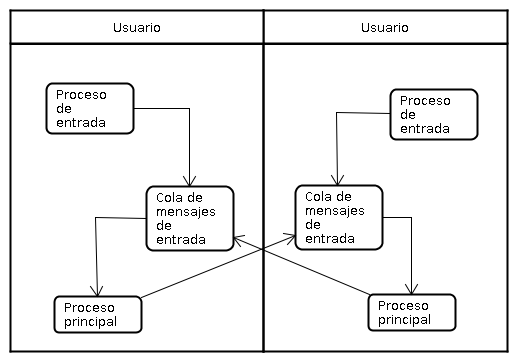
\includegraphics[scale=0.65]{./Images/ArquitecturaClienteConCliente}
\end{center}
\subsubsection{Cliente-Servicio de localización}
\begin{center}
\small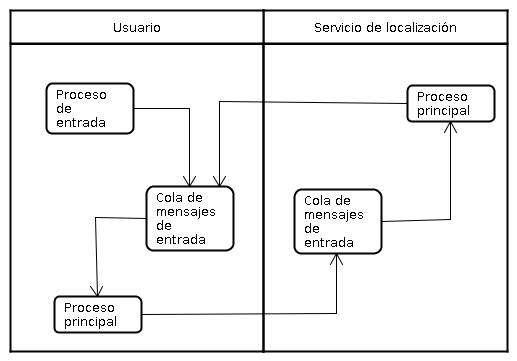
\includegraphics[scale=0.65]{./Images/ArquitecturaClienteConServidor}
\end{center}

\subsection{Diagrama de clases}
\begin{center}
\small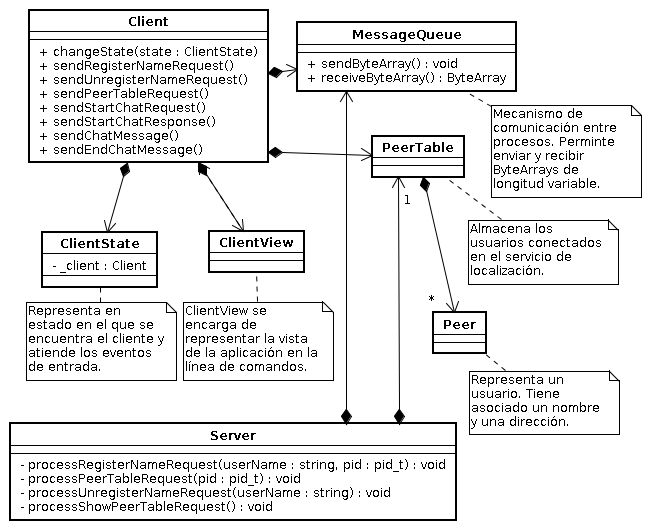
\includegraphics[scale=0.65]{./Images/DiagramaDeClases}
\end{center}

\subsection{Mensajes}

Los procesos se comunican entre sí enviandose mensajes. Se creó una entidad 
llamada ``Message'' la cual encapsula un tipo de mensaje, el id del proceso
creador y los datos asociados el mensaje. Dicho mensaje puede ser serializado
y deserializado para permitir su envio y recepción a través de la cola de mensajes.

\subsubsection{Tipos de mensajes}
\begin{itemize}
  \item {\bf TYPE NONE:} tipo de mensaje inválido.
  \item {\bf TYPE USER INPUT:} enviado desde el proceso que recibe los eventos de teclado \\
hacia el proceso principal cuando el usuario ingresa un comando.
  \item {\bf TYPE USER EXIT:} enviado desde el proceso que recibe los eventos de teclado \\
hacia el proceso principal cuando el usuario ingresa el comando de salida.
  \item {\bf TYPE REGISTER NAME REQUEST:} enviado al servicio de localización para registrar un nuevo usuario.
  \item {\bf TYPE REGISTER NAME RESPONSE:} enviado desde el servicio de localización al usuario para informar \\
si el nombre pudo ser registrado con éxito o no.
  \item {\bf TYPE UNREGISTER NAME REQUEST:} enviado al servicio de localización para desregistrar un usuario.
  \item {\bf TYPE SHOW PEER TABLE REQUEST:} enviado al servicio de localización para hacer que muestre la \\
tabla de contactos.
  \item {\bf TYPE PEER TABLE REQUEST:} enviado al servicio de localización por parte de un usuario para solicitar \\
la tabla de contactos actual.
  \item {\bf TYPE PEER TABLE RESPONSE:} enviado desde el servicio de localización al usuario como respuesta \\
de la solicitud de la tabla de contactos. 
  \item {\bf TYPE START CHAT REQUEST:} enviado entre usuarios para solicitar el comienzo de una seción de chat.
  \item {\bf TYPE START CHAT RESPONSE:} enviado entre usuarios para confirmar o rechazar el inicio de la seción de chat.
  \item {\bf TYPE END CHAT:} enviado entre usuarios para informar el fin de la seción de chat.
  \item {\bf TYPE CHAT MESSAGE:} enviado entre usuarios. Mensaje de chat.
  \item {\bf TYPE SERVER EXIT:} enviado al servicio de localización para cerrarlo remotamente.
\end{itemize}

\subsection{Estados del cliente}

Cada vez que el usuario ingresa un comando, se procesa. El significado de los mensajes o comandos
tipeados por el usuario dependen del estado en el que se encuentre la aplicación al momento de 
enviarlos. Por ejemplo, si dos usuarios se encuentran chateando, y uno usuario ingresa un comando 
``usuarios'' (visualizar la tabla de contactos) se esperaría que el usuario con el que se encuentra
chateando reciba un mensaje en texto plano con el contenido ``usuarios'' y no que visualice la
tabla de contactos en su terminal. Por esta razón, se optó por el uso del patrón de diseño ``State'' 
(o estado) el cual nos permite que cada tipo de estado sea el encargado de procesar los mensajes que llegan 
al proceso principal de cada usuario. 

\subsubsection{Diagrama de estados}
\begin{center}
\small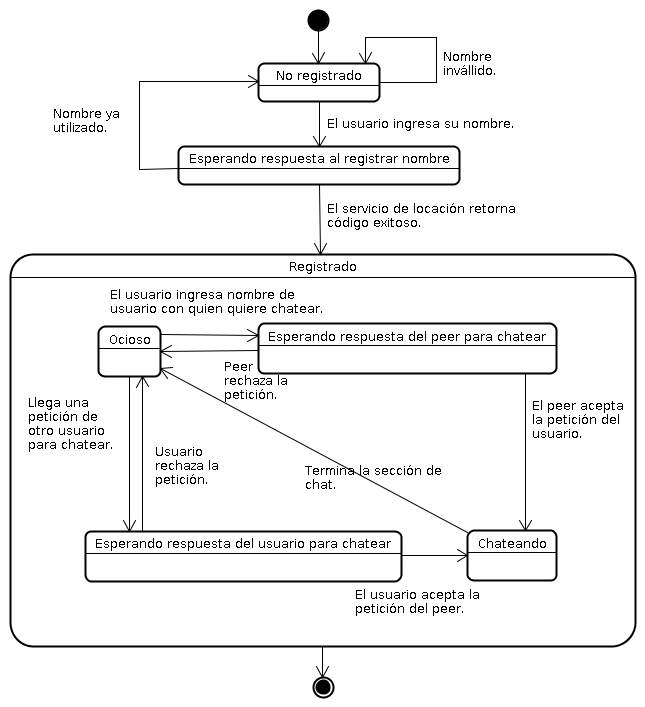
\includegraphics[scale=0.65]{./Images/DiagramaDeEstados}
\end{center}

\subsubsection{Diagrama de clases de los estados}
\begin{center}
\small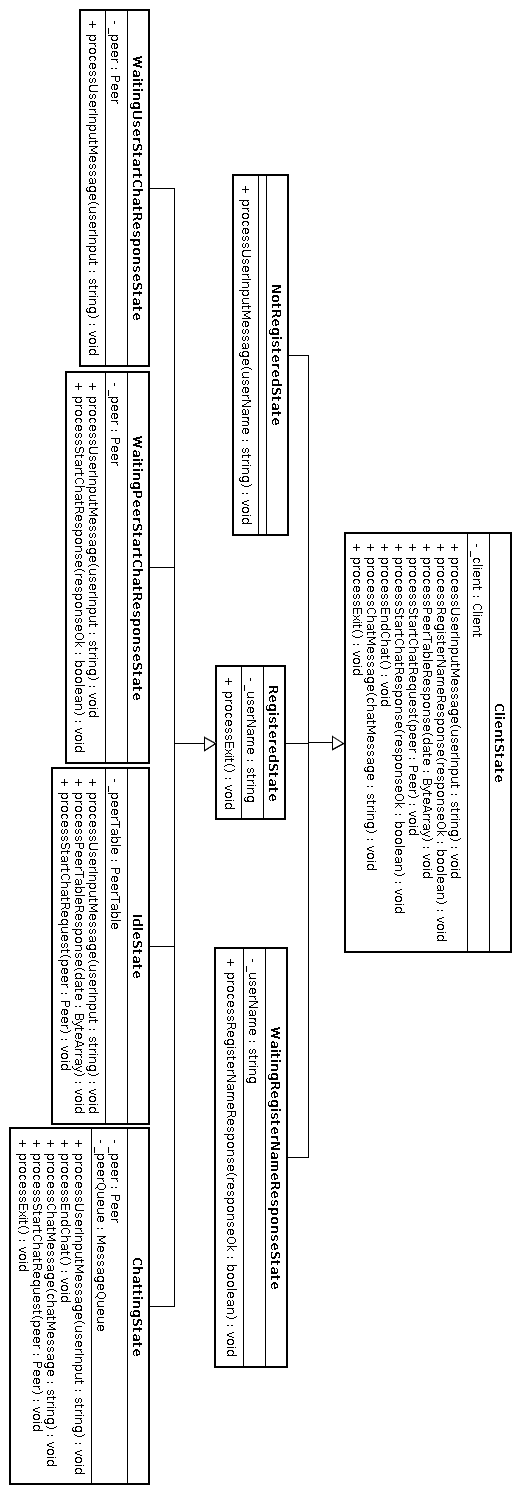
\includegraphics[scale=0.45]{./Images/DiagramaDeClasesDeLosEstados2}
\end{center}


\section{Corrida de prueba}

\begin{itemize}
  \item Opciones al correr el servicio de localización.
\end{itemize}
\begin{center}
  \small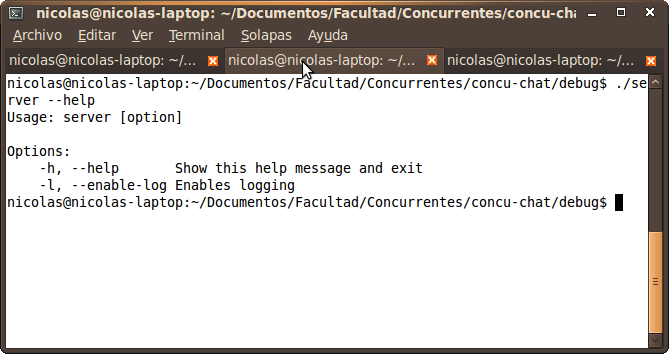
\includegraphics[scale=0.65]{./Images/AyudaServer}
\end{center}

\begin{itemize}
  \item Opciones al correr un cliente.
\end{itemize}
\begin{center}
  \small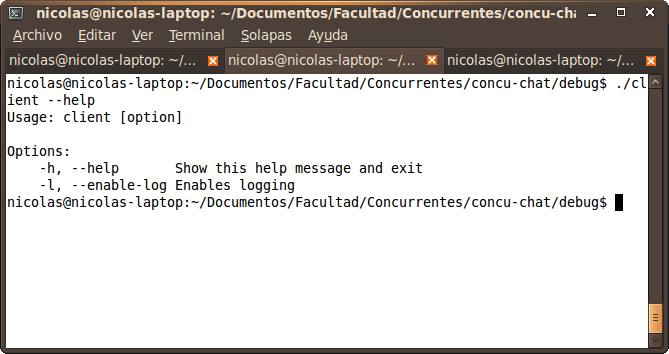
\includegraphics[scale=0.65]{./Images/AyudaCliente}
\end{center}

\begin{itemize}
  \item Correr servicio de localización.
\end{itemize}
\begin{center}
  \small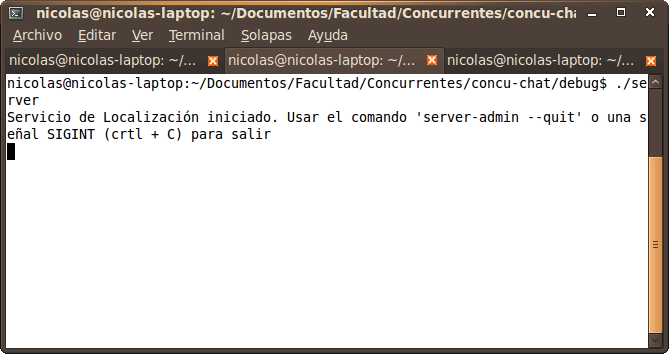
\includegraphics[scale=0.65]{./Images/Server}
\end{center}

\begin{itemize}
  \item Correr usuarios.
\end{itemize}
\begin{center}
  \small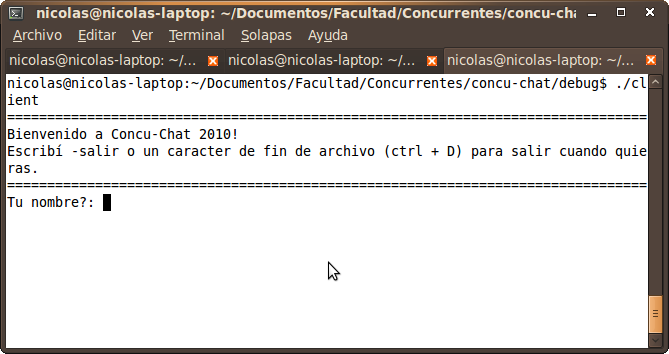
\includegraphics[scale=0.65]{./Images/Cliente}
\end{center}

\begin{itemize}
  \item Usuarios ingresan nombres.
\end{itemize}
\begin{center}
  \small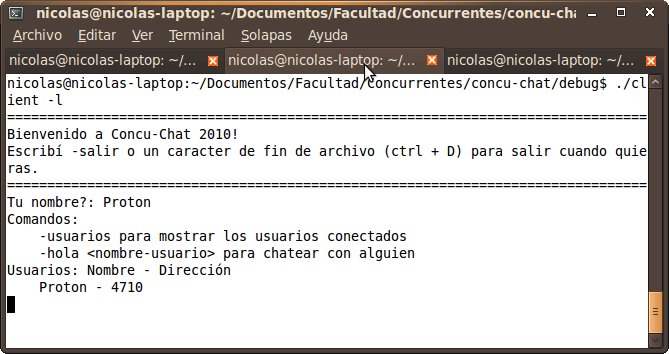
\includegraphics[scale=0.65]{./Images/Conver1}
  \small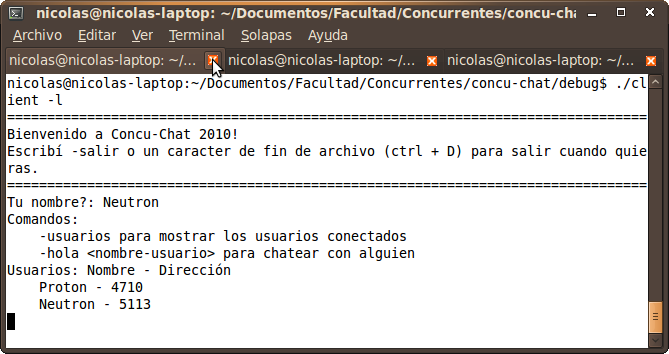
\includegraphics[scale=0.65]{./Images/Conver2}
\end{center}

\begin{itemize}
  \item Un usuario envia una petición de chat, y el otro la acepta.
\end{itemize}
\begin{center}
  \small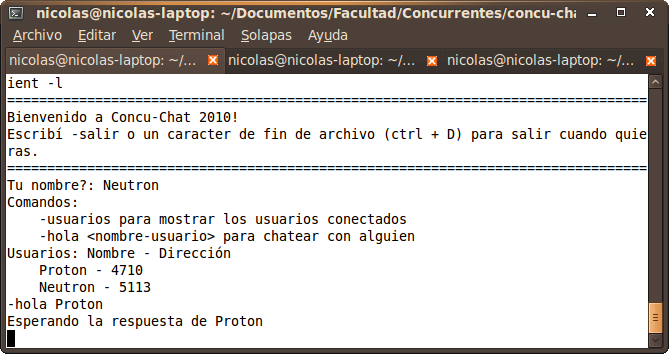
\includegraphics[scale=0.65]{./Images/Conver3}
  \small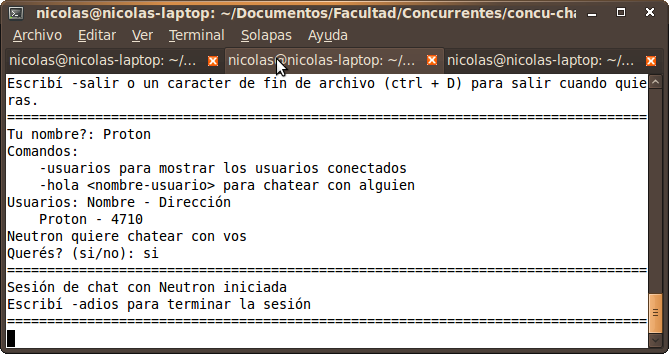
\includegraphics[scale=0.65]{./Images/Conver4}
\end{center}

\begin{itemize}
  \item Usuarios chateando.
\end{itemize}
\begin{center}
  \small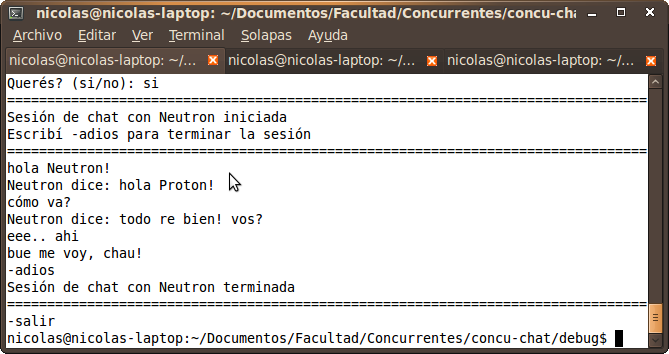
\includegraphics[scale=0.65]{./Images/Conver5}
  \small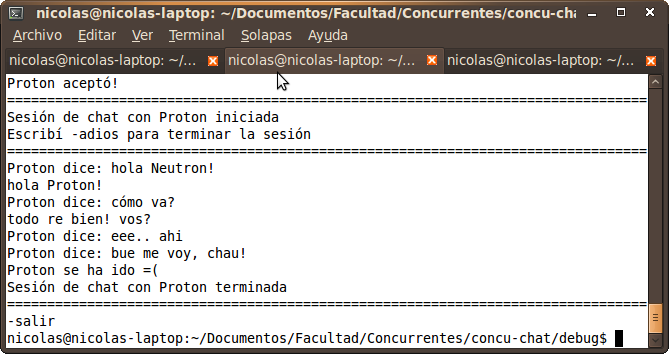
\includegraphics[scale=0.65]{./Images/Conver6}
\end{center}

\section{Conclusiones}

% ------------------------------ Fin del tp -------------------------------

\end{document}

%---------------------------- Fin del documento ---------------------------
